\section{Theorie}
\label{sec:Theorie}

Betrachtet man das Verhalten von Lichtwellen an Objekten deren Dimensionen ungefähr der Größe der Wellenlänge $\lambda$ des Lichtes entsprechen, so kann man an diesen Objekten Beugungserscheinungen feststellen.
In diesem Versuch handelt es sich dabei um unterschiedlich geartete Spalte.
Um die Brechungserscheinungen beschreiben zu können, kann zwischen zwei Arten von Beugungen unterschieden werden; der Fresnel- und der Fraunhofer-Beugung.
In diesem Versuch wird die Fraunhofersche Beugung betrachtet, da ihre Beschreibung mathematischer einfacher ist.
Die Fraunhofersche Beugung kann verwendet werden, wenn die Lichtquelle ins Unendliche, bzw. relativ zur Spaltgröße weit entfernt platziert wird.
Der Strahlengang kann dann als parallel angenommen werden.
In einem Punkt P hinter dem Spalt, z.B. auf einem Schirm, interferieren dann nur die Lichtwellen, die unter dem gleichen Winkel $\phi$ gebeugt werden.
Dies ist in Abbildung \ref{fig:Fraunhofer} dargestellt.

\begin{figure}
  \centering
  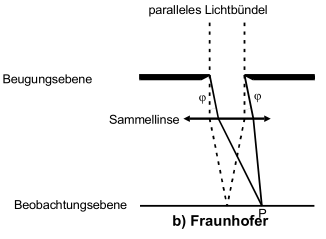
\includegraphics{images/Fraunhofer.png}
  \caption{Darstellung der Fraunhoferschen Beugung am Einzelspalt, entnommen der Versuchsanleitung \cite[31]{1}}
  \label{fig:Fraunhofer}
\end{figure}

Dieses Verhalten kann durch das Huygennssche Prinzip der Elemtarwellen und der Interferenz von Wellen erklärt werden.
Das Huygennssche Prinzip besagt, dass von jedem Punkt einer Wellenfront zu jedem Zeitpunkt neue Kugelwellen ausgehen, welche sich ebenfalls wieder überlagern und eine neue Wellenfront bilden.
Den Zustand eines beliebigen Punktes innerhalb dieses Wellenfeldes erhält man durch Überlagerung sämtlicher Elementarwellen, welche zur gleichen Zeit an diesem Punkt ankommen.
Die beobachteten Beugungserscheinungen am Spalt können somit darauf zurückgeführt werden, dass sich das Licht nach Durchtritt durch den Spalt nicht mehr nur in seine Einfallsrichtung ausbreiten kann.
Somit muss über sämtliche Elemtarwellen mit gleichem Beugungswinkel $\phi$ summiert werden.
Da es sich bei den Strahlenbündeln um infinitesimale Wellenfronten handelt, geht die Summe in eine Integration über den kompletten Spalt über.


Es wird davon ausgegangen, dass es sich bei den einfallenden Wellen um ebende Wellen der Gestalt:

\begin{equation}
  A(z,t) = A_0 \symup{exp}\left\{i \left(\omega t - 2\pi \frac{z}{\lambda} \right) \right\}
\end{equation}

handelt.
Zwei Strahlen die den Abstand x zueinander innerhalb des Spaltes aufweisen, stellt sich ein Phasenunterschied $\delta$ ein.
Dieser beträgt und ist in Abbildung \ref{fig:Phasenunterschied} dargestellt:

\begin{equation}
  \delta = \frac{2\pi x \symup{sin}(\phi)}{\lambda}
\end{equation}

\begin{figure}
  \centering
  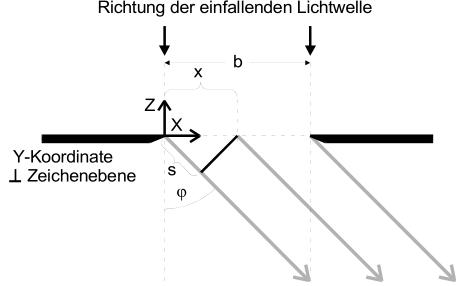
\includegraphics[scale=0.7]{images/Phasenunterschied.png}
  \caption{Der gangunterschied zweier Straheln im Einzelspalt, entnommen der Versuchsanleitung \cite[32]{1}}
  \label{fig:Phasenunterschied}
\end{figure}

Nach Ausführen der Integration und einiger Umformungen ergibt sich für die Amplitude des in $\phi$-Richtung abgelenkten Strahles:

\begin{equation}
  B(z, t, \phi) = A_0 \symup{exp}\left\{i \left(\omega t - 2\pi \frac{z}{\lambda} \right) \right\}
  \cdot \symup{exp}\left\{ \frac{i b \pi \symup{sin}(\phi)}{\lambda} \right\}
  \cdot \frac{\lambda}{\pi \symup{sin}(\phi)}
  \cdot \symup{sin} \left\{ \frac{b \pi \symup{sin}(\phi)}{\lambda} \right\}
\end{equation}

Die beiden komplexen Exponentialfunktionen stellen Phasenfunktionen dar und sind für die experimentelle Betrachtung irrelevant.
Für die Überprüfung wirde die zeitlich gemittelte Intensität $I(\phi)$ betrachtet.
Die Amplitude B lässt sich nicht direkt messen.
Hierfür wird $I(\phi) \propto B(\phi)^2$ verwendet.
Es gilt somit:

\begin{equation}
  I(\phi) \propto B(\phi)^2 =
  A_0^2 b^2 \left( \frac{\lambda}{\pi \symup{sin}(\phi)} \right)^2
  \cdot \symup{sin}^2 \left\{ \frac{b \pi \symup{sin}(\phi)}{\lambda} \right\}
\end{equation}

Ein Doppelspalt kann analog berechnet werden.
Dafür werden zwei Einzelspalte überlagert.
Der Abstand zwischen den Spalten beträgt s.
Es ergibt sich dann für die Intensitätsvertilung $I(\phi)$:

\begin{equation}
  I(\phi) \propto B(\phi)^2 =
  4 \symup{cos}^2 \left\{ \frac{s \pi \symup{sin}(\phi)}{\lambda} \right\}
  \cdot \left( \frac{\lambda}{\pi \symup{sin}(\phi)} \right)^2
  \cdot \symup{sin}^2 \left\{ \frac{b \pi \symup{sin}(\phi)}{\lambda} \right\}
\end{equation}
